% AR-Politeia Cycle 1 -- Authoritative Comprehensive Record
% Written by the Write-Comprehensive Agent from research/findings.json.
% This record intentionally contains no journal length limit. PDF is generated
% via Makefile (latexmk -pdf); the PDF itself is Git-ignored.
\documentclass[11pt,a4paper]{article}

\usepackage[T1]{fontenc}
\usepackage[utf8]{inputenc}
\usepackage{amsmath,amssymb,amsthm}
\usepackage{booktabs}
\usepackage{array}
\usepackage{graphicx}
\usepackage{tikz}
\usetikzlibrary{arrows.meta,positioning,calc,fit,backgrounds,decorations.pathreplacing}
\usepackage{pgfplots}
\pgfplotsset{compat=1.17}
\usepackage{tcolorbox}
\tcbuselibrary{skins,breakable}
\usepackage{xcolor}
\usepackage[margin=2.6cm]{geometry}
\usepackage[colorlinks=true,linkcolor=blue!55!black,citecolor=blue!55!black,urlcolor=blue!55!black]{hyperref}
\usepackage{cleveref}
\usepackage{caption}
\usepackage{enumitem}
\usepackage{microtype}

\definecolor{accent}{RGB}{20,72,130}
\definecolor{warn}{RGB}{160,40,40}
\definecolor{ok}{RGB}{20,120,70}
\definecolor{grey}{RGB}{90,90,90}

\newtcolorbox{keybox}[1][]{%
  enhanced jigsaw,
  breakable,
  colback=accent!6,
  colframe=accent,
  boxrule=1.1pt,
  arc=2.5mm,
  left=8pt,right=8pt,top=7pt,bottom=7pt,
  title={\textbf{Key finding.} #1},
  fonttitle=\bfseries\large,
  coltitle=white,
  colbacktitle=accent,
}

\newtcolorbox{warningbox}{%
  enhanced jigsaw,
  breakable,
  colback=warn!6,
  colframe=warn,
  boxrule=1.1pt,
  arc=2.5mm,
  left=8pt,right=8pt,top=7pt,bottom=7pt,
  title={\textbf{Negative / blocked result.}},
  fonttitle=\bfseries\large,
  coltitle=white,
  colbacktitle=warn,
}

\newcommand{\obs}[1]{\texttt{#1}}
\newcommand{\field}[1]{\texttt{#1}}
\newcommand{\code}[1]{\texttt{#1}}

\title{\bfseries AR-Politeia Cycle 1\\[0.35em]
\large Heterogeneous Resource Landscapes and Socioeconomic Structure:\\
A Preregistered Matched-Landscape Study of a Minimal Langevin Agent Model\\[0.5em]
\Large Authoritative Comprehensive Record (Cycle 1 Status: no confirmatory claim supported)}

\author{AutoResearcher Project \code{ar-politeia}, Cycle 1}
\date{Generated 2026-08-20 (Asia/Shanghai)}

\begin{document}
\maketitle

\begin{abstract}
This comprehensive record documents Cycle 1 of the \code{ar-politeia} research
plan. The cycle tested whether the spatial organization of a resource
landscape, holding total resources, pixel histogram, accessible area,
population, and initial wealth matched, is sufficient to change steady-state
population aggregation and wealth structure in a minimal fixed-population
Langevin agent model. The cycle is \emph{not} a positive result: the numerical
calibration gate \code{E0-NUMERICS} failed on time-step convergence and
stationarity, and all three confirmatory experiments
(\code{E1-MATCHED-LANDSCAPES}, \code{E2-CHANNEL-ABLATION},
\code{E3-ROBUSTNESS-HOLDOUT}) were hard-blocked before any confirmatory run was
executed. The claim \code{C1-NUM} is therefore \textbf{contradicted} under its
preregistered joint criteria; claims \code{C2-LANDSCAPE},
\code{C3-CHANNELS}, and \code{C4-ROBUSTNESS} are \textbf{inconclusive} because
no direct empirical evidence exists for them. The only passing diagnostics are
wealth conservation, wealth non-negativity, equal-state absorption, fixed
population, and finite metrics. This record preserves every negative and
blocked result in full, cross-checks every claim against
\code{research/findings.json}, and deliberately introduces no unsupported
scientific claim. The recommended next action is to return to the human/science
gate, repair the candidate parameter lock using only runtime and outcome-blind
health diagnostics, rerun \code{E0-NUMERICS} until all checks pass, and then
re-submit \code{E1}--\code{E3}.
\end{abstract}

\begin{keybox}[Cycle 1 status at a glance]
Cycle 1 does \textbf{not} establish any confirmatory scientific claim.
\code{E0-NUMERICS} completed 25 runs but failed its calibration gate on
\code{dt\_convergence} and \code{stationarity}; the wealth-conservation and
non-negativity checks passed. \code{E1}--\code{E3} were never executed because
the parameter lock is non-final and the \code{E0} calibration dependency failed.
Plain-language summary: \emph{we could not yet make the simulation numerically
trustworthy enough to run the landscape comparison, so the core scientific
question remains unanswered.}
\end{keybox}

\tableofcontents

%==============================================================================
\section{Introduction}
\label{sec:intro}

This section states what Cycle 1 tried to do and its bottom line. The bottom
line is negative/inconclusive: the cycle built and executed the numerical
sanity-check layer, found two calibration failures, and was correctly stopped
before any confirmatory landscape comparison.

The broad research program, \emph{AR-Politeia}, asks how heterogeneous resource
landscapes shape socioeconomic structure. Its imported predecessor attempted a
civilization-wide narrative (loyalty, hierarchy, polity classification, and
China--Europe contrasts); a code-and-evidence audit concluded that plan was
over-broad, historically confounded, and partly tautological, so it was retired
(\code{research/plan.json}, \code{revision.retired\_claims}). Cycle 1 therefore
narrows the question to one causal, generative-mechanism claim that a minimal
agent model can actually test.

The core question is stated in \code{research/question.md}: \emph{given matched
total resources, resource marginal distribution, accessible area, population,
and initial wealth, does the spatial autocorrelation of the resource landscape
change steady-state population aggregation and wealth structure?} Intuitively,
the question is whether the \emph{arrangement} of resources---not their total or
their histogram---matters once agents can move and exchange. The intended
answer is causal: clustered landscapes are compared against an exact-histogram
spatial shuffle, so any difference must come from spatial organization.

\subsection{What this record contains}

The record proceeds as follows. \Cref{sec:related} reviews related work.
\Cref{sec:model} defines the minimal model and each mechanism with its physical
intuition. \Cref{sec:design} restates the preregistered hypotheses, claims,
observables, and analysis policy. \Cref{sec:landscapes} describes the matched
landscape generator. \Cref{sec:experiments} reports every executed and blocked
experiment with figures and tables. \Cref{sec:discussion}, \Cref{sec:limits},
and \Cref{sec:conclusion} interpret the negative results, list limitations, and
give next steps. Supplementary material in
\code{paper/comprehensive/supplementary/} contains the full diagnostics and
claim--evidence crosswalk.

\section{Related Work}
\label{sec:related}

This section places the minimal model and its matched-landscape design against
three methodological anchors. Its conclusion is that the design follows
pattern-oriented modeling and uncertainty-quantification practice, but that
Cycle 1 is deliberately far smaller in inference scope than the kinetic-theory
and data-inference literature it cites.

\subsection{Kinetic theories of socioeconomic structure.}
Dur\'an-Olivencia's \emph{The Emergence of Socio-Economic Structure: A
First-Principles Kinetic Theory} (2025) proposes a fluctuation--dissipation
kinetic framework in which social aggregates are described by coarse-grained
densities and temperatures. Cycle 1 borrows the language of Langevin dynamics
and stationary distributions but \emph{does not} claim a social
fluctuation--dissipation law; \code{research/question.md} explicitly forbids
interpreting social temperature or fluctuation--dissipation as validated social
laws.

\subsection{Inference of Langevin dynamics from social data.}
Bae et al., \emph{Unveiling hidden features of social evolution by inferring
Langevin dynamics from data} (2026), infer drift and diffusion terms from
observed trajectories. Cycle 1 is complementary but generative rather than
inferential: it simulates a known dynamical law forward and tests causal
interventions (landscape shuffling and channel ablation) instead of fitting a
law backward from data.

\subsection{Pattern-oriented modeling and uncertainty quantification.}
Grimm et al. (2005) argue that agent-based models should be validated against
multiple observed patterns rather than a single scalar. McCulloch et al. (2022)
formalize uncertainty quantification for agent-based models. Cycle 1 follows
both: it preregisters several observables (resource--density correlation,
Moran's $I$, occupancy entropy, wealth Gini), requires stationarity diagnostics
before analysis, and freezes a simulation-resolution equivalence threshold
(SESOI) before confirmatory outcomes are inspected.

\subsection{Distinctness of this cycle.}
None of the cited work provides a preregistered, matched-histogram
clustered-versus-shuffled landscape contrast with a two-channel (movement and
production) $2\times2$ ablation. That design is the contribution Cycle 1
attempts to realize; because the calibration gate failed, the design remains
implemented but not yet executed.

\section{Minimal Generative Model}
\label{sec:model}

This section defines the model and explains each mechanism's physical meaning.
The conclusion first: the model keeps only position, momentum, and wealth;
turns off reproduction, death, culture, technology, loyalty, conquest, and
taxation; and couples wealth to space through two independently switchable
terrain channels---movement and production.

\subsection{State variables}

Each agent $i$ has three dynamic quantities (\code{research/hypothesis.md},
\emph{minimal state}):

\begin{equation}
\text{state}_i(t) \;=\; \bigl(x_i(t),\, y_i(t),\, p_{x,i}(t),\, p_{y,i}(t),\, w_i(t)\bigr).
\label{eq:state}
\end{equation}

Equation \eqref{eq:state} means an agent is only ``where it is, where it is
heading, and how much wealth it holds''; its ability $\epsilon_i$ is frozen to a
constant ($\epsilon=1$) in Cycle 1 and the population is fixed, so neither
ability evolution nor demography can act as a hidden confounder.

\subsection{Langevin dynamics (movement)}

Positions and momenta follow a BBK (Br\"unger--Brooks--Karplus) Langevin update
with friction $\gamma$ and temperature $T$ (\code{langevin\_integrator.cpp}):

\begin{equation}
\mathrm{d}p = F\,\mathrm{d}t - \gamma\,p\,\mathrm{d}t + \sqrt{2\gamma m k_B T}\,\mathrm{d}W,
\qquad
\frac{\mathrm{d}x}{\mathrm{d}t} = \frac{p}{m},
\label{eq:langevin}
\end{equation}

Equation \eqref{eq:langevin} says agents are pushed by the deterministic force
$F$ (terrain attraction plus, when enabled, social force), slowed by friction
$\gamma$, and kicked by thermal noise whose amplitude is set by the
fluctuation--dissipation relation. With the Cycle 1 parameters $m=1$,
$\gamma=1$, $T=0.5$, $k_B=1$, this is an overdamped-but-inertial random motion;
when $\gamma=0$ and $T=0$ it reduces to deterministic Velocity--Verlet; this
deterministic limit is a property of the integrator, not the setting of the
Cycle 1 conservation checks (which concern wealth and use the standard
$\gamma=1$, $T=0.5$ dynamics with flat terrain and production/consumption/decay
off).

The force is the gradient of a potential $V(x,y)$. The legacy fallback terrain
uses Gaussian potential wells, $F_{\mathrm{terrain}}=-\nabla V$ with

\begin{equation}
V(x,y) = -\,\sum_k \mathrm{depth}_k \exp\!\left(-\frac{(x-c_{x,k})^2+(y-c_{y,k})^2}{2\,\mathrm{width}_k^2}\right),
\label{eq:terrain-potential}
\end{equation}

where the summation runs over the Gaussian wells used by the legacy fallback
terrain; Cycle 1 itself does \emph{not} use that fallback. In Cycle 1 the
resource field $R(x,y)\ge0$ (mean $1$, minimum $0$) is converted to an
elevation field $H(x,y)=R_{\max}-R(x,y)$, so high-resource cells are
\emph{low} elevation. The movement force is then
$F=-s_F\,\nabla H=+s_F\,\nabla R$, and the production potential is
$V_{\mathrm{prod}}(x,y)=-s_P R(x,y)$.
Equation \eqref{eq:terrain-potential} is shown for the general Gaussian-well
case and means the landscape acts as attractive wells: locations with more
resource are deeper and pull agents toward them. In the grid implementation the
same intuition holds via the inverted elevation field---the force points up the
resource gradient, and this is exactly the ``movement channel'' of the
ablation.

\Cref{fig:schematic-model} summarizes the state and the three mechanisms.

\begin{figure}[htbp]
\centering
\resizebox{\textwidth}{!}{%
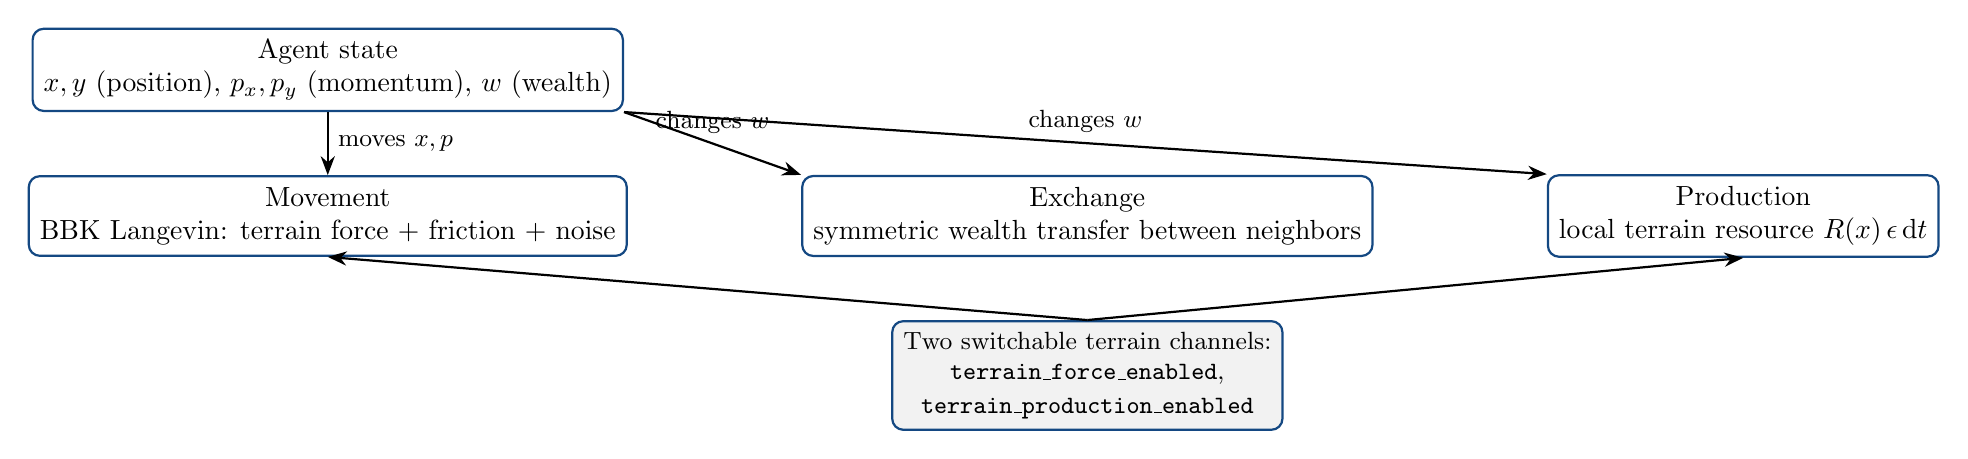
\begin{tikzpicture}[
  node distance=8mm and 7mm,
  box/.style={draw=accent, thick, rounded corners, minimum height=7mm, align=center, inner sep=4pt},
  arrow/.style={-{Stealth[length=2.4mm]}, thick},
]
  \node[box] (state) {Agent state\\ $x,y$ (position), $p_x,p_y$ (momentum), $w$ (wealth)};
  \node[box, below=of state] (langevin) {Movement\\ BBK Langevin: terrain force $+$ friction $+$ noise};
  \node[box, right=22mm of langevin] (exchange) {Exchange\\ symmetric wealth transfer between neighbors};
  \node[box, right=22mm of exchange] (prod) {Production\\ local terrain resource $R(x)\,\epsilon\,\mathrm{d}t$};
  \draw[arrow] (state.south) -- (langevin.north) node[midway,right,font=\small] {moves $x,p$};
  \draw[arrow] (state.south east) -- (exchange.north west) node[midway,above,font=\small] {changes $w$};
  \draw[arrow] (state.south east) -- (prod.north west) node[midway,above,font=\small] {changes $w$};
  \node[box, fill=grey!8, below=of exchange, font=\small, align=center] (channels) {Two switchable terrain channels:\\ \code{terrain\_force\_enabled},\\[1pt] \code{terrain\_production\_enabled}};
  \draw[arrow] (channels.north) -- (langevin.south);
  \draw[arrow] (channels.north) -- (prod.south);
\end{tikzpicture}
}
\caption{\textbf{Model schematic.} The three columns left-to-right are the three
dynamic channels---movement, exchange, and production---and the top box is the
minimal state. The key observation is that terrain enters through exactly two
switchable channels (movement force and local production), which is the
structure later ablated in \code{E2-CHANNEL-ABLATION}. The conclusion is that
any landscape effect must be attributable to one or both of these channels,
never to an unmodeled ``topology'' term.}
\label{fig:schematic-model}
\end{figure}

\subsection{Symmetric resource exchange}

Wealth transfers occur between neighboring pairs within the interaction range.
The rule is label-symmetric and saturating
(\code{resource\_exchange.cpp}):

\begin{equation}
A_i = \epsilon_i\,\frac{w_i}{w_i+w_{\mathrm{ref}}},\qquad
\Delta w = \eta\,\frac{A_i-A_j}{A_i+A_j}\,\min(w_i,w_j),
\label{eq:exchange}
\end{equation}

where $\eta$ is the exchange rate, $w_{\mathrm{ref}}$ is the wealth
half-saturation scale ($w_{\mathrm{ref}}=5$ in Cycle 1), and the transfer is
taken from $j$ and given to $i$ (the code updates $w_i \leftarrow w_i+\Delta w$,
$w_j \leftarrow w_j-\Delta w$). Equation \eqref{eq:exchange} means richer
agents gain in pairwise encounters while poorer agents lose, but the rule is
antisymmetric under relabeling, so aggregate wealth is conserved and inequality
is produced by state differences rather than by a biased rule. The
saturation factor $w/(w+w_{\mathrm{ref}})$ makes ability sublinear in wealth and
prevents the transfer from diverging at large wealth.

\Cref{fig:schematic-exchange} illustrates the transfer.

\begin{figure}[htbp]
\centering
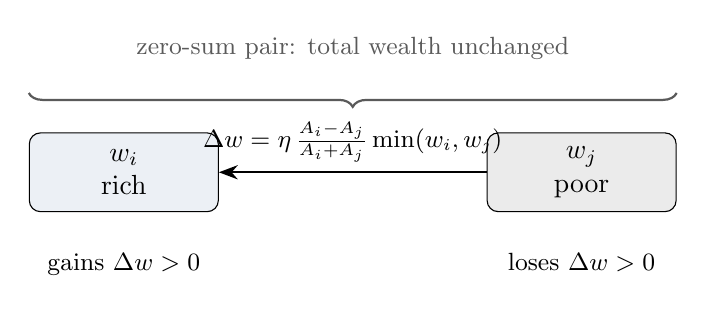
\begin{tikzpicture}[
  box/.style={draw, rounded corners, minimum width=24mm, minimum height=10mm, align=center, inner sep=3pt},
  arrow/.style={-{Stealth[length=2.4mm]}, thick},
]
  \node[box, fill=accent!8] (i) {$w_i$\\ rich};
  \node[box, fill=grey!12, right=34mm of i] (j) {$w_j$\\ poor};
  \draw[arrow] (j) -- node[above,font=\small] {$\Delta w=\eta\,\frac{A_i-A_j}{A_i+A_j}\min(w_i,w_j)$} (i);
  \node[below=4mm of i, font=\small] {gains $\Delta w>0$};
  \node[below=4mm of j, font=\small] {loses $\Delta w>0$};
  \draw[decorate,decoration={brace,amplitude=5pt}, thick, grey] ($(j.north east)+(0,5mm)$) -- node[above=3mm,font=\small] {zero-sum pair: total wealth unchanged} ($(i.north west)+(0,5mm)$);
\end{tikzpicture}
\caption{\textbf{Symmetric exchange schematic.} The left-to-right axis is the
wealth ordering of the two agents; the arrow is the transfer of wealth from the
poorer to the richer agent when their abilities differ. The key observation is
that the magnitude is bounded by $\eta\min(w_i,w_j)$ and the pair update is
zero-sum. The conclusion is that the exchange kernel conserves total wealth by
construction and cannot itself create negative wealth in a single pairwise
update, consistent with the \code{E0-NUMERICS} conservation and non-negativity
checks.}
\label{fig:schematic-exchange}
\end{figure}

\subsection{Terrain channels and resource production}

Wealth changes through production, consumption, and decay
(\code{resource\_exchange.cpp}):

\begin{equation}
\mathrm{d}w_i = R(x_i)\,\epsilon_i\,\mathrm{d}t - c\,\mathrm{d}t - d\,w_i\,\mathrm{d}t,
\qquad
R(x)=\mathrm{base\_production}\cdot\mathrm{scale}\cdot\max(0,-V(x)),
\label{eq:production}
\end{equation}

where $c$ is the consumption rate and $d$ the proportional decay rate. Equation
\eqref{eq:production} means each agent earns from the local resource depth
$\max(0,-V(x))$, pays a fixed consumption cost, and loses a fraction of wealth
to depreciation; in Cycle 1 the confirmatory parameter set uses
$\mathrm{base\_production}=0.01$, $c=0$, $d=0$, so only the terrain-dependent
production term is active. The two switchable channels are
\code{terrain\_force\_enabled} (whether the terrain gradient moves agents) and
\code{terrain\_production\_enabled} (whether the terrain depth produces
wealth).

\subsection{Simulation simplifications}

Cycle 1 disables every module that could confound the landscape comparison
(\code{research/plan.json}, \code{scope.disabled\_modules}): culture,
technology jumps, reproduction, mortality, plague, loyalty, conquest, taxation,
and polity classification are all off; population is fixed. This means the only
ways a landscape can affect the measured observables are the movement channel,
the production channel, and their interaction through wealth exchange.

\section{Research Design and Preregistered Claims}
\label{sec:design}

This section restates the preregistered design. The conclusion is that the
design was causal and falsifiable, and that the negative outcomes in
\Cref{sec:experiments} are design-respecting stops rather than post-hoc
interpretations.

\subsection{Hypotheses}

\code{research/hypothesis.md} declares four hypotheses. $H_0$: spatial
organization has no effect beyond numerical and random fluctuation once the
resource marginals and total are matched. $H_1$: high-autocorrelation clustered
landscapes change the resource--density association, the spatial aggregation
scale of density, and the steady wealth distribution relative to an
exact-histogram spatial shuffle. $H_2$: the effect decomposes into a movement
channel and a production channel whose main effects and interaction are
estimated by a $2\times2$ factorial ablation. $H_3$: if $H_1$ holds, the effect
direction is consistent across population sizes, grid resolutions, and
held-out landscape families, with confidence intervals excluding the
preregistered minimal effect.

\subsection{Claims}

The four machine-checked claims are listed in \Cref{tab:claims}. Their verdicts
come from \code{research/findings.json} and are mirrored in
\code{research/orchestration/comprehensive.json} and
\code{paper/comprehensive/claims.json}.

\begin{table}[htbp]
\centering
\begin{tabular}{@{}lp{6.4cm}p{2.0cm}@{}}
\toprule
\textbf{Claim} & \textbf{Text} & \textbf{Verdict} \\
\midrule
\code{C1-NUM} & minimal model conserves wealth, stays non-negative, and main observables converge in time step under non-degenerate small perturbations & \textbf{contradicted} \\
\code{C2-LANDSCAPE} & matched clustered landscapes produce population-spatial-structure differences beyond numerical noise relative to spatially shuffled landscapes & \textbf{inconclusive} \\
\code{C3-CHANNELS} & landscape effect decomposes into movement $\times$ production $2\times2$ main and interaction effects & \textbf{inconclusive} \\
\code{C4-ROBUSTNESS} & core effect direction is consistent across population sizes, grid resolutions, and held-out landscape families & \textbf{inconclusive} \\
\bottomrule
\end{tabular}
\caption{\textbf{Preregistered claims and their Cycle 1 verdicts.} Columns are
claim identifier, claim text, and the verdict carried in
\code{research/findings.json}. The key observation is that only
\code{C1-NUM} has executed evidence and it is contradicted; the other three
have no executed confirmatory evidence. The conclusion is that the cycle ended
at the numerical-calibration layer.}
\label{tab:claims}
\end{table}

\subsection{Observables}

The primary observable is the steady-window Spearman rank correlation between
the resource field and the binned population density
(\code{resource\_density\_spearman\_rho}). Co-primary observables are the
global Moran's $I$ of the density field (\code{density\_morans\_i}) and the
normalized Shannon occupancy entropy (\code{occupancy\_entropy}). Secondary
observables are wealth Gini, wealth variance, total-wealth relative drift,
integrated autocorrelation time, and effective sample size. Each observable's
formula is defined in \code{landscape\_study.py} and reproduced in the
supplementary.

\subsection{Confirmatory analysis policy}

The analysis unit is a paired random seed across matched landscapes. Effects
are paired mean differences with 10\,000-sample bootstrap 95\% intervals and
100\,000-sample paired sign-flip $p$-values; multiplicity is controlled by Holm
correction within each metric family. The equivalence rule freezes a SESOI from
paired same-seed $\mathrm{d}t/2$-versus-$\mathrm{d}t/4$ discretization
differences in \code{E0-NUMERICS} before any \code{E1}--\code{E3} outcome is
inspected; it is a simulation-resolution limit, not a substantive social-science
effect size. Failed runs are reported and rerun only under the declared failure
policy; no seed is replaced after outcomes are observed.

\section{Landscape Generation and Matching}
\label{sec:landscapes}

This section describes how clustered and shuffled landscapes are constructed and
machine-checked. The conclusion is that the matching is exact at input
generation time: the shuffled field is a pixel permutation of the clustered
field, so total resources and the pixel histogram coincide by construction.

The generator (\code{landscape\_study.py}) creates a clustered field as a sum
of five anisotropic Gaussian bumps with lognormal amplitudes, then subtracts
the minimum and normalizes the mean to one. The shuffled control is the exact
pixel permutation of the clustered field; the flat control is a constant field
equal to the mean. \Cref{fig:matched} sketches the construction. For each seed,
an audit (\code{audit\_matched\_landscapes}) checks equal shape, exact sorted
histogram equality, non-negativity and finiteness, and total-resource agreement
within $10^{-12}$ relative tolerance; the executed audits for \code{E0} and
\code{B0} all passed.

\begin{figure}[htbp]
\centering
\resizebox{\textwidth}{!}{%
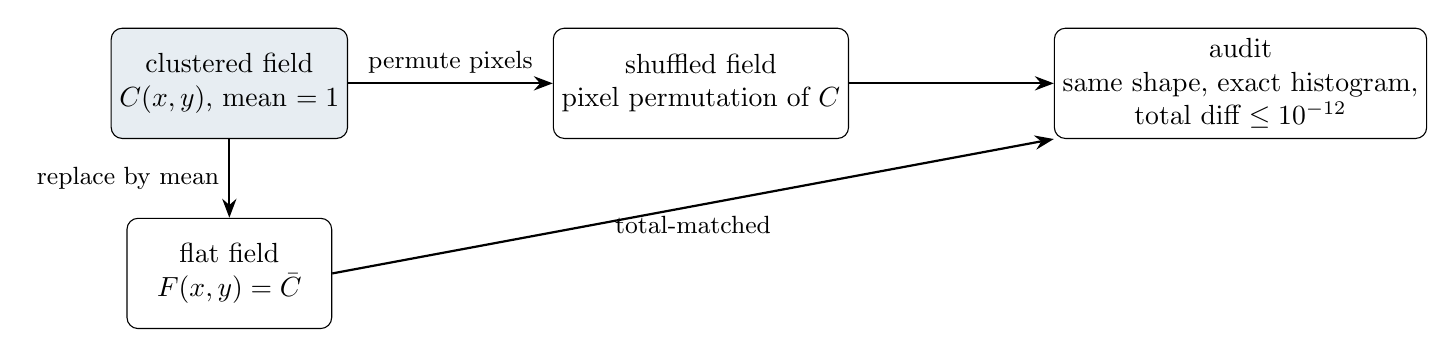
\begin{tikzpicture}[
  box/.style={draw, rounded corners, minimum width=26mm, minimum height=14mm, align=center, inner sep=3pt},
  arrow/.style={-{Stealth[length=2.4mm]}, thick},
]
  \node[box, fill=accent!10] (clustered) {clustered field\\ $C(x,y)$, mean $=1$};
  \node[box, below=10mm of clustered] (flat) {flat field\\ $F(x,y)=\bar C$};
  \node[box, right=26mm of clustered] (shuffled) {shuffled field\\ pixel permutation of $C$};
  \node[box, right=26mm of shuffled] (audit) {audit\\ same shape, exact histogram,\\ total diff $\le 10^{-12}$};
  \draw[arrow] (clustered) -- node[above,font=\small] {permute pixels} (shuffled);
  \draw[arrow] (shuffled) -- (audit);
  \draw[arrow] (clustered) -- node[left,font=\small] {replace by mean} (flat);
  \draw[arrow] (flat.east) -- node[below,font=\small] {total-matched} (audit.south west);
\end{tikzpicture}
}
\caption{\textbf{Matched-landscape construction.} The top-left-to-top-right flow
shows the clustered field and its exact pixel permutation (shuffled); the
downward branch shows the total-matched flat field. The key observation is that
the shuffled control preserves the pixel histogram and total exactly, so only
spatial autocorrelation differs. The conclusion is that any
clustered-minus-shuffled difference is attributable to spatial arrangement, not
to total or histogram mismatch.}
\label{fig:matched}
\end{figure}

\section{Experiments and Results}
\label{sec:experiments}

This section reports every experiment, executed or blocked, with the exact
numbers from the corresponding \code{result.json} files. The conclusion first:
two experiments executed and both failed their preregistered health/calibration
gates; three confirmatory experiments were hard-blocked before producing any
numerical result.

\subsection{Experiment manifest and hardware}
\label{sec:manifest}

\Cref{tab:manifest} lists each experiment, its role, run configuration, and
Cycle 1 status. \Cref{tab:params} gives the full shared parameter table.

\begin{table}[htbp]
\centering
\small
\begin{tabular}{@{}lp{4.0cm}p{3.9cm}p{2.5cm}@{}}
\toprule
\textbf{ID} & \textbf{Role} & \textbf{Configured runs} & \textbf{Status} \\
\midrule
\code{B0-DYNAMICS-PILOT} & runtime/health pilot (non-evidentiary) & 3 seeds, clustered-active only & \textbf{completed, gate failed} \\
\code{E0-NUMERICS} & numerical calibration + SESOI & 5 seeds $\times$ 5 conditions $=25$ & \textbf{completed, gate failed} \\
\code{E1-MATCHED-LANDSCAPES} & clustered vs shuffled vs flat & 20 seeds $\times$ 4 conditions $=80$ & \textbf{blocked} \\
\code{E2-CHANNEL-ABLATION} & $2\times2$ channel ablation & 20 seeds $\times$ 2 landscapes $\times$ 4 channel states $=160$ & \textbf{blocked} \\
\code{E3-ROBUSTNESS-HOLDOUT} & scale/resolution/holdout robustness & 10 seeds $\times$ 3 populations $\times$ 2 grids $\times$ 2 families & \textbf{blocked} \\
\bottomrule
\end{tabular}
\caption{\textbf{Experiment manifest.} Columns are experiment identifier, role
in the design, configured number of runs, and Cycle 1 status. The key
observation is that only the two non-confirmatory or calibration layers
executed; all confirmatory layers are blocked. The conclusion is that Cycle 1
stopped before the scientific question could be answered.}
\label{tab:manifest}
\end{table}

\begin{table}[htbp]
\centering
\small
\begin{tabular}{@{}llll@{}}
\toprule
\textbf{Parameter} & \textbf{Value} & \textbf{Parameter} & \textbf{Value} \\
\midrule
domain bounds & $[0,100]\times[0,100]$ & time step $\mathrm{d}t$ & $0.01$ \\
temperature $T$ & $0.5$ & friction $\gamma$ & $1.0$ \\
social strength & $0.0$ (off) & interaction range & $2.5$ \\
exchange rate $\eta$ & $0.003$ & ability saturation $w_{\mathrm{ref}}$ & $5.0$ \\
base production & $0.0$ (E0), $0.01$ (others) & consumption rate $c$ & $0.0$ \\
wealth decay rate $d$ & $0.0$ & mean wealth & $5.0$ \\
terrain force scale & $1.0$ & terrain production scale & $1.0$ \\
OpenMP threads & $8$ & GPU & $0$ \\
\bottomrule
\end{tabular}
\caption{\textbf{Shared physical and numerical parameters.} The two columns
repeat parameter/value pairs for readability. The key observation is that
friction and temperature are active but social force, consumption, decay, and
population dynamics are off in the confirmatory regime. The conclusion is that
the model is a minimal inertial Langevin system with terrain channels and
saturating wealth exchange, as defined in \Cref{sec:model}.}
\label{tab:params}
\end{table}

The execution environment (\code{jobs/*/env.txt}) is host \code{umi} (4$\times$
NVIDIA A100-40GB; no GPU used), Debian, Python 3.11.2, NumPy 2.4.4, SciPy
1.17.1, CMake 3.25.1, g++ 12.2.0, OpenMP with 8 threads, and source commit
\code{029820d0161941b88cbf73580f0ccc557608a392}.

\subsection{B0-DYNAMICS-PILOT}
\label{sec:b0}

\emph{What this subsection does and its conclusion:} it reports the
runtime/health pilot, whose stationarity gate failed for all three seeds while
wealth non-negativity, fixed population, and finite metrics passed. The pilot
is non-evidentiary and has no shuffled control, so it cannot support any
landscape-effect claim.

The pilot ran three clustered-active landscapes at population $N=500$ and
$64\times64$ resolution for total time $100.0$ with 12 steady-window snapshots.
Its result file is \code{research/jobs/B0-DYNAMICS-PILOT/result.json} and the
raw per-run metrics are in
\code{research/jobs/B0-DYNAMICS-PILOT/workspace/replicate\_metrics.csv}.

\begin{table}[htbp]
\centering
\small
\begin{tabular}{@{}lp{1.9cm}p{2.6cm}p{1.1cm}p{4.6cm}@{}}
\toprule
\textbf{Check} & \textbf{Threshold} & \textbf{Observed} & \textbf{Pass} & \textbf{\code{result.json} field} \\
\midrule
all runs stationary & all runs pass & false (3/3 fail) & \textbf{no} & \code{raw\_metrics\_summary.all\_runs\_stationary} \\
wealth non-negative & $\ge -10^{-12}$ & $\min=2.8550564\times10^{-7}$ & yes & \code{raw\_metrics\_summary.wealth\_nonnegative} \\
population constant & $=N$ & $\min=\max=500.0$ & yes & \code{raw\_metrics\_summary.population\_constant} \\
metrics finite & all finite & finite & yes & \code{raw\_metrics\_summary.metrics\_finite} \\
\bottomrule
\end{tabular}
\caption{\textbf{B0 dynamics-health gate.} Columns are check, threshold,
observed value, pass/fail, and the exact \code{result.json} field. The key
observation is that the only failing check is stationarity; wealth
non-negativity, fixed population, and finiteness all pass. The conclusion is
that the candidate parameter set is numerically safe but not yet stationary
within the preregistered window.}
\label{tab:b0-gate}
\end{table}

\Cref{tab:b0-stationarity} reports the stationarity diagnostics per seed.

\begin{table}[htbp]
\centering
\small
\begin{tabular}{@{}llllll@{}}
\toprule
\textbf{Seed} & \textbf{rho drift} & \textbf{Moran drift} & \textbf{entropy drift} & \textbf{Gini drift} & \textbf{var drift} \\
\midrule
7103 & $0.5421$ & $0.8744$ & $0.00725$ & $0.6544$ & $1.0136$ \\
7207 & $0.1846$ & $1.0241$ & $0.0120$ & $0.5762$ & $0.9908$ \\
7309 & $0.8359$ & $0.9640$ & $0.0214$ & $0.5688$ & $0.9853$ \\
\bottomrule
\end{tabular}
\caption{\textbf{B0 normalized window drift per seed and observable.} Rows are
seeds, columns are normalized steady-window drifts (dimensionless; the
preregistered maximum is $0.1$) from
\code{workspace/stationarity\_report.json}. The key observation is that
resource--density correlation, Moran's $I$, wealth Gini, and wealth variance
all exceed the $0.1$ drift ceiling for every seed, while occupancy entropy
passes. The conclusion is that the system has not reached the preregistered
steady window in $T=100$.}
\label{tab:b0-stationarity}
\end{table}

\begin{warningbox}
\code{B0-DYNAMICS-PILOT} failed its stationarity gate for all three seeds
($7103$, $7207$, $7309$). This is recorded in full, not softened. It is a
dynamics-health failure, not a scientific null result about landscapes.
\end{warningbox}

\subsection{E0-NUMERICS}
\label{sec:e0}

\emph{What this subsection does and its conclusion:} it reports the numerical
calibration layer, which completed 25 runs and passed conservation,
non-negativity, and equal-state absorption but failed time-step convergence and
stationarity, so the frozen SESOI is not authorized for confirmatory use.

The experiment used five seeds ($1103,2207,3301,4409,5519$) and five conditions
per seed: \code{equal-no-exchange}, \code{equal-exchange}, and three
\code{perturbed-dt} factors ($1.0,0.5,0.25$) on a flat landscape with
$\mathrm{d}t=0.01$ (factors scale to $0.01$, $0.005$, $0.0025$). Its result file
is \code{research/jobs/E0-NUMERICS/result.json} and the calibration is
\code{research/jobs/E0-NUMERICS/numerical\_calibration.json}.

\Cref{tab:e0-gate} reproduces the five calibration checks digit-for-digit.

\begin{table}[htbp]
\centering
\small
\begin{tabular}{@{}lp{1.7cm}p{2.9cm}p{1.0cm}p{3.5cm}@{}}
\toprule
\textbf{Check} & \textbf{Threshold} & \textbf{Observed} & \textbf{Pass} & \textbf{Field} \\
\midrule
wealth conservation & $\le 10^{-8}$ & $2.511028287699446\times10^{-9}$ & yes & \code{max\_absolute\_wealth\_drift} \\
wealth non-negative & $\ge -10^{-12}$ & $5.1766245\times10^{-41}$ & yes & \code{minimum\_wealth} \\
$\mathrm{d}t$ convergence & all main obs $\le 0.02$ & Gini change $0.26584885869833064$ & \textbf{no} & \code{dt\_half\_vs\_quarter\_mean\_absolute\_change.wealth\_gini} \\
equal state absorbing & $\le 10^{-20}$ & max wealth variance $0.0$ & yes & \code{equal\_exchange\_max\_wealth\_variance} \\
stationarity & all runs pass & \code{false} & \textbf{no} & \code{stationarity\_pass} \\
\bottomrule
\end{tabular}
\caption{\textbf{E0 numerical-calibration gate.} Columns are check, preregistered
threshold, observed value, pass/fail, and the exact \code{numerical\_calibration.json}
field. The key observation is that the two failures are $\mathrm{d}t$
convergence (driven by wealth Gini) and stationarity; conservation,
non-negativity, and equal-state absorption pass. The conclusion is that
\code{C1-NUM} is contradicted as a joint claim even though its conservation
component is individually true.}
\label{tab:e0-gate}
\end{table}

\Cref{tab:e0-dt} gives the $\mathrm{d}t/2$-versus-$\mathrm{d}t/4$ mean absolute
changes used both for the convergence check and for the frozen SESOI.

\begin{table}[htbp]
\centering
\small
\begin{tabular}{@{}llll@{}}
\toprule
\textbf{Observable} & \textbf{Mean abs change} & \textbf{Convergence limit} & \textbf{Frozen SESOI} \\
\midrule
\code{resource\_density\_spearman\_rho} & $0.0$ & $0.02$ & $1\times10^{-6}$ \\
\code{density\_morans\_i} & $0.008572825641811355$ & $0.02$ & $0.02483292987625197$ \\
\code{occupancy\_entropy} & $0.0011749233757867516$ & $0.02$ & $0.002883297084384684$ \\
\code{wealth\_gini} & $0.26584885869833064$ & $0.02$ & $0.2811818304868519$ \\
\bottomrule
\end{tabular}
\caption{\textbf{E0 discretization convergence and frozen SESOI.} Columns are
observable, paired $\mathrm{d}t/2$-vs-$\mathrm{d}t/4$ mean absolute change,
the convergence limit, and the frozen simulation-resolution SESOI (all
dimensionless). The key observation is that wealth Gini changes by
$0.2658$ between resolutions, far above the $0.02$ limit, so the wealth
distribution is not converged at this step size. The conclusion is that the
frozen SESOI cannot yet serve as a confirmatory equivalence threshold; it is
reported here only as the attempted calibration value.}
\label{tab:e0-dt}
\end{table}

\Cref{tab:e0-runs} lists the final steady-window values per run, extracted
exactly from \code{replicate\_metrics.csv}; the full 25-row CSV is preserved in
the job workspace.

\begin{table}[htbp]
\centering
\small
\begin{tabular}{@{}llllll@{}}
\toprule
\textbf{Run} & \textbf{Gini} & \textbf{Variance} & \textbf{Min wealth} & \textbf{Gini drift} & \textbf{Pass} \\
\midrule
seed-1103--equal-no-exchange & $0.0$ & $0.0$ & $5.0$ & $0.0$ & no \\
seed-1103--equal-exchange & $0.0$ & $0.0$ & $5.0$ & $0.0$ & no \\
seed-1103--perturbed-dt-1 & $0.10203773080569478$ & $1.4784841650605485$ & $2.471151\times10^{-4}$ & $1.0160$ & no \\
seed-1103--perturbed-dt-0.5 & $0.364598856723039$ & $14.1899754623276$ & $4.5008089\times10^{-15}$ & $1.0167$ & no \\
seed-1103--perturbed-dt-0.25 & $0.6201324647972065$ & $42.51454356276534$ & $1.8129234\times10^{-38}$ & $0.6085$ & no \\
seed-2207--equal-no-exchange & $0.0$ & $0.0$ & $5.0$ & $0.0$ & no \\
seed-2207--equal-exchange & $0.0$ & $0.0$ & $5.0$ & $0.0$ & no \\
seed-2207--perturbed-dt-1 & $0.10492111391522696$ & $1.5217560160200345$ & $1.9933729\times10^{-3}$ & $1.0147$ & no \\
seed-2207--perturbed-dt-0.5 & $0.3696474296083716$ & $14.805504932193532$ & $9.7213598\times10^{-16}$ & $1.0234$ & no \\
seed-2207--perturbed-dt-0.25 & $0.6317572980235273$ & $44.42474394674785$ & $9.6852395\times10^{-36}$ & $0.5574$ & no \\
seed-3301--equal-no-exchange & $0.0$ & $0.0$ & $5.0$ & $0.0$ & no \\
seed-3301--equal-exchange & $0.0$ & $0.0$ & $5.0$ & $0.0$ & no \\
seed-3301--perturbed-dt-1 & $0.10193259153711715$ & $1.609699680835066$ & $1.2817956\times10^{-9}$ & $1.0210$ & no \\
seed-3301--perturbed-dt-0.5 & $0.3612375533962144$ & $14.417545982501135$ & $1.434259\times10^{-21}$ & $1.0201$ & no \\
seed-3301--perturbed-dt-0.25 & $0.6270569238594541$ & $44.395229094048474$ & $3.5468381\times10^{-38}$ & $0.6024$ & no \\
seed-4409--equal-no-exchange & $0.0$ & $0.0$ & $5.0$ & $0.0$ & no \\
seed-4409--equal-exchange & $0.0$ & $0.0$ & $5.0$ & $0.0$ & no \\
seed-4409--perturbed-dt-1 & $0.10771952648408462$ & $1.6152771963273564$ & $2.4682044\times10^{-5}$ & $1.0149$ & no \\
seed-4409--perturbed-dt-0.5 & $0.36648856554561327$ & $14.46854488408937$ & $1.10324\times10^{-17}$ & $1.0197$ & no \\
seed-4409--perturbed-dt-0.25 & $0.6365919067767616$ & $46.40950691049406$ & $3.8866753\times10^{-34}$ & $0.5773$ & no \\
seed-5519--equal-no-exchange & $0.0$ & $0.0$ & $5.0$ & $0.0$ & no \\
seed-5519--equal-exchange & $0.0$ & $0.0$ & $5.0$ & $0.0$ & no \\
seed-5519--perturbed-dt-1 & $0.09903203077263689$ & $1.4333291096423562$ & $4.2027981\times10^{-5}$ & $1.0053$ & no \\
seed-5519--perturbed-dt-0.5 & $0.34125525673327384$ & $12.72597571267837$ & $8.1596046\times10^{-18}$ & $1.0249$ & no \\
seed-5519--perturbed-dt-0.25 & $0.6169333620412158$ & $41.61644184299551$ & $5.1766245\times10^{-41}$ & $0.6058$ & no \\
\bottomrule
\end{tabular}
\caption{\textbf{E0 per-run final steady-window values.} Columns are run
identifier, wealth Gini, wealth variance, minimum wealth, normalized Gini
window drift, and the stationarity pass flag, all taken verbatim from
\code{workspace/replicate\_metrics.csv}. The key observation is that equal
initial conditions remain at Gini $0$ while perturbed initial conditions evolve
to Gini between $0.099$ and $0.637$ with a systematic $\mathrm{d}t$ dependence,
and no run passes stationarity. The conclusion is that the wealth distribution
is both non-stationary and discretization-sensitive in the tested window,
which is exactly the failure recorded in the calibration gate.}
\label{tab:e0-runs}
\end{table}

\begin{figure}[htbp]
\centering
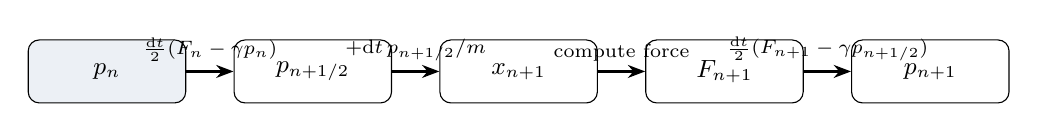
\begin{tikzpicture}[
  box/.style={draw, rounded corners, minimum width=20mm, minimum height=8mm, align=center, inner sep=2pt, font=\small},
  arrow/.style={-{Stealth[length=2.2mm]}, thick},
]
  \node[box, fill=accent!8] (p0) {$p_n$};
  \node[box, right=6mm of p0] (ph) {$p_{n+1/2}$};
  \node[box, right=6mm of ph] (x1) {$x_{n+1}$};
  \node[box, right=6mm of x1] (f1) {$F_{n+1}$};
  \node[box, right=6mm of f1] (p1) {$p_{n+1}$};
  \draw[arrow] (p0) -- node[above,font=\scriptsize] {$\frac{\mathrm{d}t}{2}(F_n-\gamma p_n)$} (ph);
  \draw[arrow] (ph) -- node[above,font=\scriptsize] {$+\mathrm{d}t\,p_{n+1/2}/m$} (x1);
  \draw[arrow] (x1) -- node[above,font=\scriptsize] {compute force} (f1);
  \draw[arrow] (f1) -- node[above,font=\scriptsize] {$\frac{\mathrm{d}t}{2}(F_{n+1}-\gamma p_{n+1/2})$} (p1);
\end{tikzpicture}
\caption{\textbf{BBK integration step.} The left-to-right axis is the sequence
of a single time step: current momentum, half-step momentum, new position, new
force, and updated momentum. The key observation is that each step is a
momentum--position--force--momentum sequence that reduces to Velocity--Verlet
when $\gamma=0$ and noise is off. The conclusion is that the integrator is
reduces to Velocity--Verlet in the deterministic limit; the wealth-conservation
check in \code{E0-NUMERICS} does not rely on that limit but instead follows
from the zero-sum exchange update with production, consumption, and decay
switched off.}
\label{fig:bbk}
\end{figure}

\begin{keybox}[E0 calibration gate failed]
\code{E0-NUMERICS} completed 25 runs but did \textbf{not} pass its calibration
gate: \code{dt\_convergence} failed (wealth Gini changes by $0.2658$ between
$\mathrm{d}t/2$ and $\mathrm{d}t/4$) and \code{stationarity} failed. Therefore
\code{C1-NUM} is contradicted and the frozen SESOI is not authorized for
confirmatory use.
\end{keybox}

\subsection{E1-MATCHED-LANDSCAPES}
\label{sec:e1}

\emph{What this subsection does and its conclusion:} it documents that the
confirmatory matched-landscape comparison was prepared but hard-blocked before
execution, so \code{C2-LANDSCAPE} has no direct empirical evidence.

\code{E1-MATCHED-LANDSCAPES} was configured for 20 seeds $\times$ 4 conditions
(\code{clustered}, \code{shuffled}, \code{flat}, \code{clustered-no-exchange})
at $N=2000$ and $128\times128$ resolution. Its result file is
\code{research/jobs/E1-MATCHED-LANDSCAPES/result.json}, which reports
\code{status: "blocked"}, \code{pass: false}, and \code{jobctl\_reconcile:
"failed"} with exit code 1. The declared gates are
\code{parameter\_lock\_final=false},
\code{parameter\_lock\_status="candidate\_pending\_non\_evidentiary\_runtime\_pilot\_and\_e0"},
and \code{e0\_calibration\_pass=false}. The input audit and run specifications
exist, but \code{replicate\_metrics.csv}, effect estimates, and stationarity
reports are missing by design of the abort.

\begin{table}[htbp]
\centering
\small
\begin{tabular}{@{}lll@{}}
\toprule
\textbf{Field} & \textbf{Value} & \textbf{Source} \\
\midrule
status & \code{"blocked"} & \code{result.json.status} \\
pass & \code{false} & \code{result.json.pass} \\
jobctl exit code & $1$ & \code{result.json.jobctl\_exit\_code} \\
jobctl reconcile & \code{"failed"} & \code{result.json.jobctl\_reconcile} \\
parameter lock final & \code{false} & \code{result.json.gates.parameter\_lock\_final} \\
E0 calibration pass & \code{false} & \code{result.json.gates.e0\_calibration\_pass} \\
replicate metrics & missing & \code{result.json.artifact\_status} \\
\bottomrule
\end{tabular}
\caption{\textbf{E1 blocked status.} Columns are field, recorded value, and the
exact \code{result.json} location. The key observation is that the block is a
deterministic upstream gate failure, not a failed run. The conclusion is that
no matched-landscape effect estimate exists for \code{C2-LANDSCAPE}.}
\label{tab:e1-block}
\end{table}

\subsection{E2-CHANNEL-ABLATION}
\label{sec:e2}

\emph{What this subsection does and its conclusion:} it documents that the
$2\times2$ channel ablation was prepared but hard-blocked, so
\code{C3-CHANNELS} has no channel effect estimates.

\code{E2-CHANNEL-ABLATION} was configured for 20 seeds $\times$ 2 landscapes
(\code{clustered}, \code{shuffled}) $\times$ 4 channel states
(force$\times$production on/off) $=160$ runs. Its result file reports
\code{status: "blocked"} with the same two gate failures as \code{E1};
\code{channel\_effects.json} and \code{replicate\_metrics.csv} are missing.
\Cref{fig:channels} shows the preregistered $2\times2$ design, which remains
valid and ready to run once the upstream gates pass.

\begin{figure}[htbp]
\centering
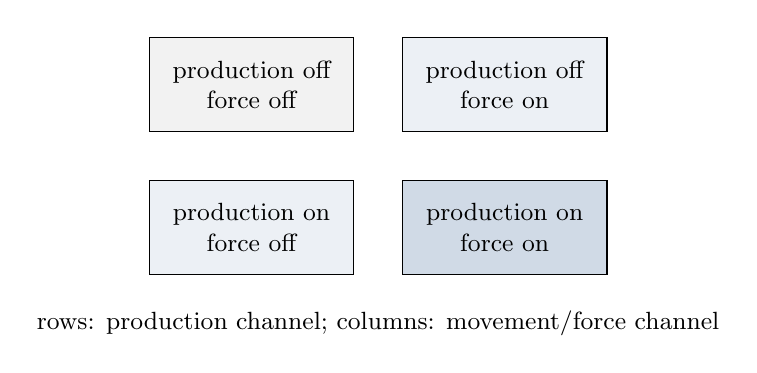
\begin{tikzpicture}[
  cell/.style={draw, minimum width=26mm, minimum height=12mm, align=center, inner sep=2pt, font=\small},
]
  \matrix (m) [row sep=6mm, column sep=6mm] {
    \node[cell, fill=grey!8] {production off\\ force off}; &
    \node[cell, fill=accent!8] {production off\\ force on}; \\
    \node[cell, fill=accent!8] {production on\\ force off}; &
    \node[cell, fill=accent!20] {production on\\ force on}; \\
  };
  \node[below=2mm of m, font=\small, align=center] {rows: production channel; columns: movement/force channel};
\end{tikzpicture}
\caption{\textbf{Preregistered $2\times2$ channel ablation.} The horizontal axis
is the movement (terrain-force) channel and the vertical axis is the production
channel, each on or off. The key observation is that all four cells are
specified before outcomes, so main effects and the interaction are separable.
The conclusion is that the design can attribute a landscape effect to movement,
production, or their interaction---but no such run was executed in Cycle 1.}
\label{fig:channels}
\end{figure}

\begin{table}[htbp]
\centering
\small
\begin{tabular}{@{}lll@{}}
\toprule
\textbf{Field} & \textbf{Value} & \textbf{Source} \\
\midrule
status & \code{"blocked"} & \code{result.json.status} \\
jobctl exit code & $1$ & \code{result.json.jobctl\_exit\_code} \\
parameter lock final & \code{false} & \code{result.json.gates.parameter\_lock\_final} \\
E0 calibration pass & \code{false} & \code{result.json.gates.e0\_calibration\_pass} \\
channel effects & missing & \code{result.json.artifact\_status} \\
\bottomrule
\end{tabular}
\caption{\textbf{E2 blocked status.} Columns are field, recorded value, and the
exact \code{result.json} location. The key observation is that the runner
aborted before producing channel effect estimates. The conclusion is that
\code{C3-CHANNELS} is inconclusive, not contradicted.}
\label{tab:e2-block}
\end{table}

\subsection{E3-ROBUSTNESS-HOLDOUT}
\label{sec:e3}

\emph{What this subsection does and its conclusion:} it documents that the
robustness/holdout stage was prepared but hard-blocked by its dependencies, so
\code{C4-ROBUSTNESS} has no scale- or holdout-family evidence.

\code{E3-ROBUSTNESS-HOLDOUT} was configured for populations
$\{2000,5000,10000\}$, grid shapes $\{128,256\}$, and holdout families
\code{gaussian\_mixture} and \code{correlated\_random\_field} across 10 seeds.
Its result file reports \code{status: "blocked"} with the upstream dependencies
\code{E0} failed, \code{E1} blocked, and \code{E2} blocked.

\begin{table}[htbp]
\centering
\small
\begin{tabular}{@{}lll@{}}
\toprule
\textbf{Dependency} & \textbf{Status} & \textbf{Source} \\
\midrule
\code{E0-NUMERICS} & completed, \code{pass:false} & \code{result.json.dependencies.E0-NUMERICS} \\
\code{E1-MATCHED-LANDSCAPES} & blocked, \code{pass:false} & \code{result.json.dependencies.E1-MATCHED-LANDSCAPES} \\
\code{E2-CHANNEL-ABLATION} & blocked, \code{pass:false} & \code{result.json.dependencies.E2-CHANNEL-ABLATION} \\
\code{holdout\_effects.json} & missing & \code{result.json.artifact\_status} \\
\bottomrule
\end{tabular}
\caption{\textbf{E3 dependency status.} Columns are dependency, recorded status,
and the exact \code{result.json} location. The key observation is that all three
upstream requirements are unmet or blocked. The conclusion is that
\code{C4-ROBUSTNESS} is inconclusive.}
\label{tab:e3-block}
\end{table}

\section{Claim-to-Evidence Crosswalk}
\label{sec:crosswalk}

This section maps every claim to the exact evidence files used, so no claim
depends on prose memory. The conclusion is that \code{C1-NUM} is contradicted
by executed evidence and \code{C2}--\code{C4} are inconclusive because their
evidence files record blocked status.

\begin{table}[htbp]
\centering
\small
\begin{tabular}{@{}llp{7.6cm}@{}}
\toprule
\textbf{Claim} & \textbf{Verdict} & \textbf{Evidence paths} \\
\midrule
\code{C1-NUM} & contradicted &
\code{research/jobs/E0-NUMERICS/result.json}\newline
\code{research/jobs/E0-NUMERICS/numerical\_calibration.json}\newline
\code{research/jobs/E0-NUMERICS/workspace/numerical\_calibration.json}\newline
\code{research/jobs/E0-NUMERICS/workspace/stationarity\_report.json}\newline
\code{research/jobs/E0-NUMERICS/workspace/replicate\_metrics.csv} \\
\code{C2-LANDSCAPE} & inconclusive &
\code{research/jobs/E1-MATCHED-LANDSCAPES/result.json}\newline
\code{research/jobs/E3-ROBUSTNESS-HOLDOUT/result.json}\newline
\code{research/parameter\_lock.json} \\
\code{C3-CHANNELS} & inconclusive &
\code{research/jobs/E2-CHANNEL-ABLATION/result.json}\newline
\code{research/parameter\_lock.json} \\
\code{C4-ROBUSTNESS} & inconclusive &
\code{research/jobs/E3-ROBUSTNESS-HOLDOUT/result.json}\newline
\code{research/parameter\_lock.json} \\
\bottomrule
\end{tabular}
\caption{\textbf{Claim-to-evidence crosswalk.} Columns are claim, verdict, and
the exact evidence paths mirrored from \code{research/findings.json}. The key
observation is that \code{C1-NUM} has five executed artifacts and
\code{C2}--\code{C4} have only blocked-result and parameter-lock artifacts. The
conclusion is that no claim is asserted beyond its evidence.}
\label{tab:crosswalk}
\end{table}

\section{Discussion}
\label{sec:discussion}

This section interprets the negative results. The conclusion is that Cycle 1
did not fail scientifically; it stopped at the calibration gate exactly as the
design requires, and the failures themselves are informative about the model.

The conservation and non-negativity checks passing means the exchange kernel's
core bookkeeping is correct: total wealth is preserved to
$2.51\times10^{-9}$ relative drift and no wealth becomes negative in the tested
regime. The equal-state check passing means a uniform-wealth configuration is
an absorbing state of the deterministic exchange kernel, consistent with the
symmetric rule.

The two failures are distinct and actionable. The stationarity failure in both
\code{B0} and \code{E0} means the preregistered steady window (drift $\le0.1$
and effective samples $\ge$ threshold) is not reached in the allocated time; the
wealth Gini and variance in particular continue to drift. The
$\mathrm{d}t$-convergence failure means the wealth distribution is sensitive to
time-step halving at $\mathrm{d}t=0.01$, with Gini moving from about $0.10$ at
$\mathrm{d}t=0.01$ to about $0.62$--$0.64$ at $\mathrm{d}t=0.0025$ for the
perturbed initial conditions. Plain-language summary: \emph{the simulation
bookkeeping is sound, but the wealth dynamics have not settled down and still
depend on how finely time is sliced, so it is premature to measure a landscape
effect.}

Because \code{E1}--\code{E3} were blocked before execution, there is no
evidence for or against $H_1$, $H_2$, or $H_3$. The important scientific
consequence is negative but useful: the candidate parameter lock must be
revised using only runtime, numerical-stability, and outcome-blind health
diagnostics; observed \code{E1}--\code{E3} effects must not be used to amend it
(\code{research/parameter\_lock.json}, \code{amendment\_policy}).

\section{Limitations}
\label{sec:limits}

This section lists real, non-empty limitations. The conclusion is that every
scientific interpretation in this record is bounded by the calibration failure
and the blocked confirmatory stage.

\begin{itemize}[leftmargin=1.9em]
\item \textbf{No confirmatory evidence.} \code{E1}--\code{E3} were not executed,
so no statement about the core scientific question ($H_1$) or the channel
decomposition ($H_2$, $H_3$) is warranted.
\item \textbf{Non-stationary wealth dynamics.} The preregistered stationarity
gate failed in both executed experiments; all wealth-related steady-window
statistics are therefore provisional.
\item \textbf{Discretization sensitivity.} Wealth Gini differs by $0.2658$
between $\mathrm{d}t/2$ and $\mathrm{d}t/4$, so the model has not demonstrated
time-step convergence for the wealth observable.
\item \textbf{Non-final parameter lock.} The candidate lock is
\code{candidate\_pending\_non\_evidentiary\_runtime\_pilot\_and\_e0}; no
confirmatory parameter set is authorized.
\item \textbf{Unusable SESOI.} The frozen SESOI was computed but is not
authorized as a confirmatory threshold while \code{dt\_convergence} fails.
\item \textbf{Synthetic-only scope.} Even in a future passing cycle, the
evidence boundary is synthetic generative mechanism only; no claim about
specific civilizations, states, empires, or historical causation is permitted.
\item \textbf{Fixed $\epsilon$ and disabled modules.} The conclusions cannot
speak to ability evolution, demography, culture, loyalty, or institutions,
because those modules are intentionally off in Cycle 1.
\item \textbf{Limited seeds and configurations.} Executed evidence comes from
3 pilot seeds and 25 calibration runs; the larger 80/160-run confirmatory
designs remain unused.
\end{itemize}

\section{Conclusion}
\label{sec:conclusion}

Cycle 1 of \code{ar-politeia} produced a correct, honest stop: the minimal
model's exchange bookkeeping passes conservation and non-negativity checks, but
the wealth dynamics fail the preregistered stationarity and time-step
convergence gates, so the confirmatory landscape experiments were correctly
blocked. Claim \code{C1-NUM} is contradicted; \code{C2}--\code{C4} are
inconclusive. The recommended next action is stated in
\code{research/orchestration/cycle-output.json}: return to the human/science
gate, revise the candidate parameter lock using only runtime and outcome-blind
health diagnostics, rerun \code{E0-NUMERICS} until conservation,
non-negativity, $\mathrm{d}t$-convergence, and stationarity all pass, then
re-submit \code{E1}--\code{E3}.

\section*{Acknowledgments}
This record was generated by the AutoResearcher \code{write\_comprehensive}
node from \code{research/findings.json} and
\code{research/orchestration/cycle-output.json}. It did not run experiments and
introduced no new evidence.

\appendix
\section{Supplementary Material}
\label{sec:supplementary}

The complete diagnostics, full proofs, and an expanded claim--evidence map are
in \code{paper/comprehensive/supplementary/}. The repository also preserves
every machine artifact under \code{research/jobs/<exp\_id>/}. The numerical
experiments were executed only on host \code{umi}, per project rules.

\end{document}
